For over a decade, the {\sc osprey} software package~\cite{OSPREY,minDEE,OSPREY_MIE} has offered the protein design community a unique combination of continuous flexibility modeling, ensemble modeling, and algorithms with provable guarantees.  Having begun as a software release for the $K^*$ algorithm~\cite{minDEE,GrsA-LeuA}, which approximates binding constants using ensemble modeling, it now boasts a wide array of algorithms found in no other software.  {\sc osprey} has been used in many designs that were empirically successful---\textit{in vitro}~\cite{VRC07_enhance,CFTR,runx1_cbfb,GrsA-LeuA,DHFR-PNAS,GrsA-TyrA,specific_probes} and \textit{in vivo}~\cite{VRC07_enhance,CFTR,runx1_cbfb,DHFR-PNAS} as well as in non-human primates~\cite{VRC07_enhance}.  {\sc osprey}'s predictions have been validated by a wide range of experimental methods, including binding assays, enzyme kinetics and activity assays, in cell assays (MICs, fitness) and viral neutralization, {\em in vivo} studies, and crystal structures~\cite{DHFR-PNAS2, VRC07_enhance}.    

However, as {\sc osprey} grew to include more algorithms and features (Fig.~\ref{flowchart}), the code became increasingly complicated and difficult to maintain.  The growing complexity of the software also hindered its ease-of-use. {\sc osprey} 3.0 represents a complete refactoring of the code, and presents a simpler and more intuitive interface that makes protein redesign much easier than before. The new, developer-friendly code organization also facilitates adding new features to the free and open-source \osprey project, both by ourselves and by other contributors.  We have introduced a convenient Python scripting interface and added support for GPU acceleration of the bulk of the computation, allowing designs to be completed much more quickly and easily than in previous versions of {\sc osprey}.  We believe {\sc osprey} 3.0 will be a very useful tool for both developers and users of provably accurate protein design algorithms.  


\begin{figure}
\center
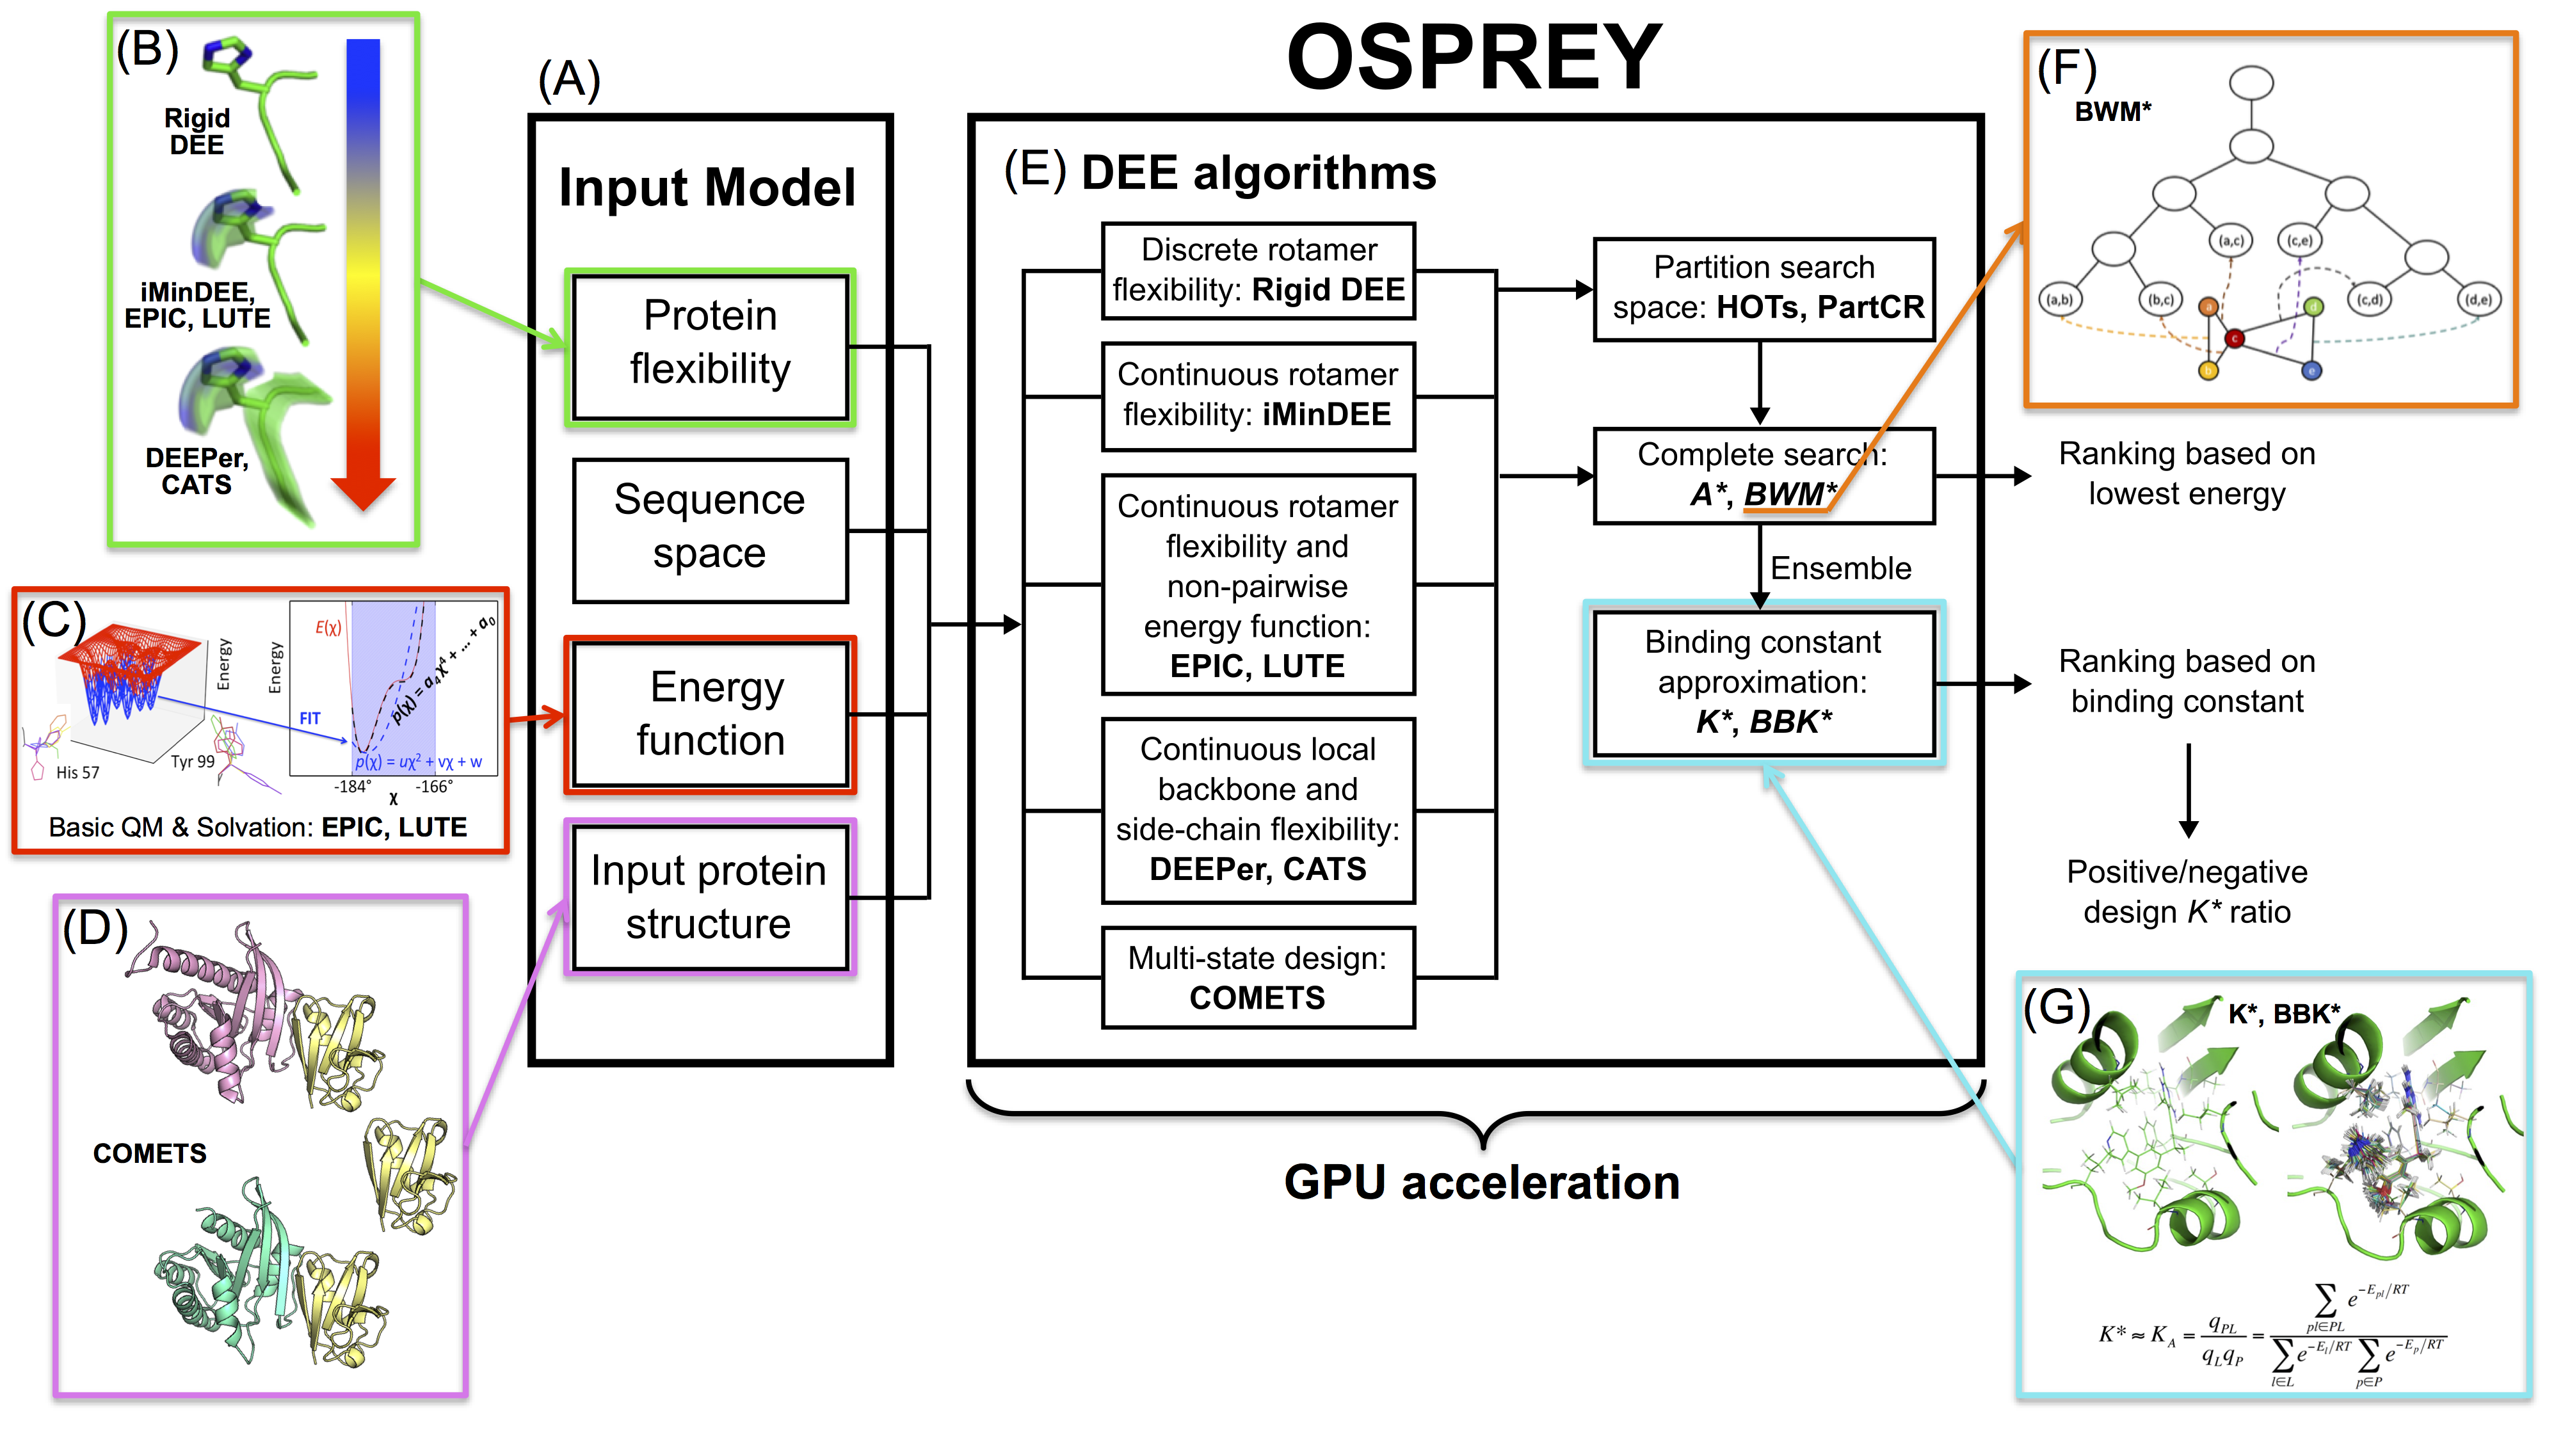
\includegraphics[width=6in]{figures/osprey_mantra.png}
 \vspace{-0.3in}%to fit the figure on one page
\caption{The \osprey protein redesign suite. (A) The input model includes a 3D structure of the protein to be redesigned, a definition of the sequence space, the allowed protein flexibility (including the rotamer library), and a pairwise energy function. (B) Rigid DEE~\cite{DEE,DEE/A*}, iMinDEE~\cite{iMinDEE}, EPIC~\cite{EPIC}, LUTE~\cite{LUTE_RECOMB}, DEEPer~\cite{DEEPer}, and CATS~\cite{CATS} model different types of protein flexibility. Flexibility ranges in difficulty from complete rigidity to continuous side chain flexibility to complete flexibility including continuous backbone flexibility. (C) The EPIC~\cite{EPIC} and LUTE~\cite{LUTE_RECOMB} algorithms also expand energy function capability by allowing for non-pairwise, basic QM and solvation. (D) COMETS~\cite{COMETS} allows for multi-state design by comparing various bound and unbound states. This allows for multiple input structures. (E) These algorithms are implemented in OSPREY and improved through the use of GPU acceleration. According to the allowed flexibility, OSPREY runs a specific pruning algorithm followed by the \as search algorithm. The \as output generates a ranking based on either the lowest-energy structure of each sequence, or an ensemble of structures computed by the \ks algorithm. (F) The \bwmstar~\cite{BWM*} algorithm takes advantage of sparse trees and branch decomposition to outperform traditional \as. (G) The \ks~\cite{K*,minDEE} algorithm calculates a \ks score (an approximation of the binding constant, $K_a$) by provably estimating the partition function for the protein, the ligand, and the protein-ligand complex. \ks also exploits a thermodynamic ensemble of structures as opposed to a single structure as illustrated in the panel (PDB ID: 3FQC). \ks can also be used to find sequences that have a high affinity for one ligand (positive design) while having a low affinity for another (negative design) by taking a ratio of \ks scores~\cite{DHFR-PNAS,DHFR-PNAS2}. }
\label{flowchart}
\end{figure}

\jccsubsection{Past successes of {\sc osprey}}

{\sc osprey} has been used for an impressive number of empirically successful designs, ranging from enzyme design to antibody design to prediction of antibiotic resistance mutations.  Notably, {\sc osprey} has been successful in many~\textit{prospective} experimental studies, i.e., studies in which our designed sequences are tested experimentally, thus validating \osprey through use in practice rather than simply through a retrospective comparison of OSPREY calculations to previous experimental results.  {\sc osprey} is most applicable to problems that can be posed in terms of biophysical state transitions like binding, allowing the $K^*$ algorithm and its variants to predict the optimal sequences based on an estimate of binding free energy computed using Boltzmann-weighted conformational ensembles.  Moreover, most protein design problems can be posed in this way, sometimes in terms of binding to more than one ligand.  \osprey is capable of both~\textit{positive design}, in which binding of a designed protein to a target is increased, and~\textit{negative design}, in which binding to a target is decreased, as well as more complicated design objectives where specific binding to one target and not to another is required.  

For example, we have successfully predicted novel resistance mutations to new inhibitors in MRSA (methicillin-resistant~\textit{Staphylococcus aureus}) using multistate design (combining negative and positive design).  \osprey does this by searching for sequences that have impaired drug binding compared to wild-type DHFR, but still form the enzyme-substrate complex as usual, allowing catalysis to proceed~\cite{DHFR-PNAS,DHFR-PNAS2}.  Our predictions were validated not only biochemically and structurally, but also at an organismal level~\cite{DHFR-PNAS2, mimb_resistance}.  Similarly, we have successfully changed the preferred substrate of an enzyme---the phenylalanine adenylation domain of gramicidin S synthetase---from phenylalanine to leucine by modeling of the two enzyme-substrate complexes, searching for sequences with improved binding to leucine and reduced binding to phenylalanine~\cite{GrsA-LeuA}.  The resulting designer enzymes exhibited improved catalysis, and designs changing the specificity from phenlyalanine to several charged amino acids were successful as well~\cite{GrsA-LeuA}.  The combination of positive and negative design in \osprey has also successfully designed mutants of the gp120 surface protein of HIV that bind specifically to particular classes of antibodies, enabling their use as probes for detecting and isolating those antibodies from human sera~\cite{specific_probes}.  

Further successes of {\sc osprey} have involved improving positive design, e.g., the interaction of the anti-HIV antibody VRC07 with its antigen, gp120.  Using this approach, we collaborated with the NIH Vaccine Research Center to design a broadly neutralizing antibody (VRC07-523LS) against HIV with unprecedented breadth and potency that is now in clinical trials (Clinical Trial Identifier: NCT03015181~\cite{VRC07_enhance,clinical605}).  We also have designed allosteric inhibitors for the leukemia-associated protein-protein interaction between Runx1 and CBF$\beta$~\cite{runx1_cbfb}.  Similarly, we have used {\sc osprey} to develop peptide inhibitors of CAL, a protein involved in cystic fibrosis~\cite{CFTR}.  

In addition, a number of other research groups have successfully used the {\sc osprey} algorithms and software (by themselves) to perform biomedically important protein designs, {\em e.g.,} to design anti-HIV antibodies that are easier to induce \cite{Georgiev:2014aa}; to design a soluble prefusion closed HIV-1-Env trimer with reduced CD4 affinity and improved immunogenicity~\cite{Gwo-yu17}; to design a transmembrane Zn$^{2+}$-transporting four-helix bundle~\cite{Joh14}; to optimize stability and immunogenicity of therapeutic proteins \cite{Parker:2013aa,Salvat:2015aa,Zhao:2015aa}; and to design sequence diversity in a virus panel and predict the epitope specificities of antibody responses to HIV-1 infection~\cite{polyclonal17}.

We believe {\sc osprey} 3.0 will enable an even greater range of successful designs.  
